\begin{surferPage}[Sestica (30 Cuspidi)]{La Sestica di Barth con 30 Cuspidi} 
   Dopo aver costruito la sestica con il massimo numero possibile di singolarit\`a ($65$, si veda un'altra superficie in questa galleria) e dopo che due dei suoi studenti di dottorato ebbero costruito nuove superfici record per gradi pi\`u alti, Wolf Barth cominci\`o a considerare la questione del numero massimo di cuspidi su superfici di un dato grado.

   La costruzione di Barth della sestica con $65$ singolarit\`a di tipo $A_1^{+-}$ (coni doppi) pu\`o essere adattata alle cuspidi; in questo modo se ne ottengono $30$: 
    \[P_6 - \alpha \cdot K^3=0,\]
  dove $P_6$ sono gli stessi piani di simetria dell'icosaedro, come nell'altra Sestica di Barth. Come prima, $K$ \`e l'equazione di una sfera unitaria:
    \vspace*{-0.4em}
    \begin{center}
      \begin{tabular}{c@{\ }c@{\ }c@{\ }c}
        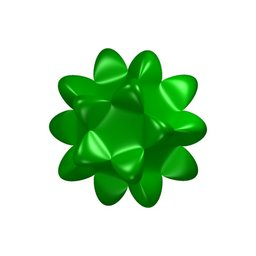
\includegraphics[height=1.2cm]{./../../common/images/barthsextic_30A2}
        &
        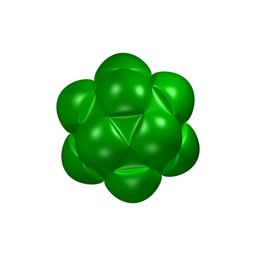
\includegraphics[height=1.2cm]{./../../common/images/barthsextic_30A2_3}
        &
        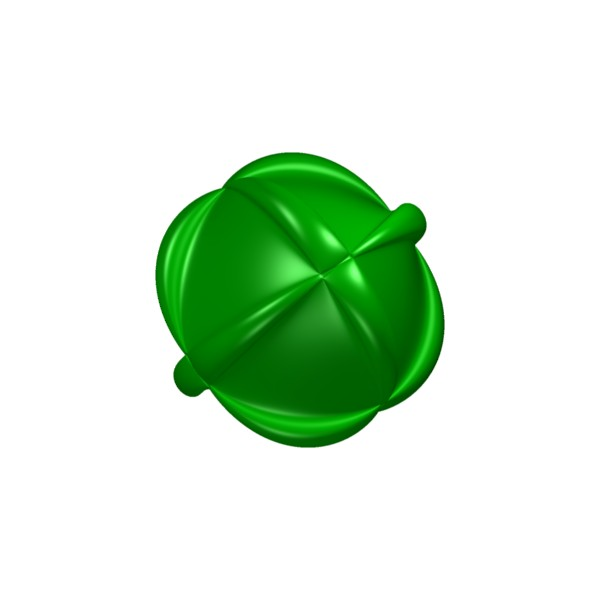
\includegraphics[height=1.2cm]{./../../common/images/barthsextic_30A2_5}
        &
        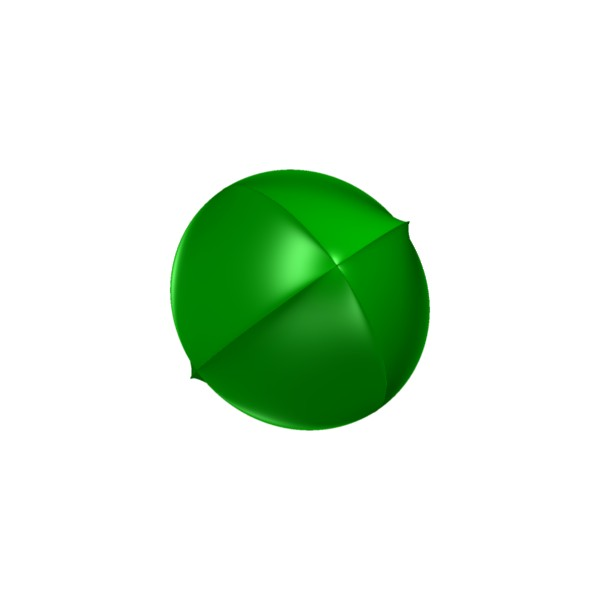
\includegraphics[height=1.2cm]{./../../common/images/barthsextic_30A2_6}
      \end{tabular}
    \end{center}    
    \vspace*{-0.3em}
     Questo \`e l'attuale record mondiale per il numero massimo di cuspidi reali su sestiche; per le cuspidi complesse, esso \`e $36$.
\end{surferPage}
